\documentclass{icmmcm}
\usepackage{graphicx} % For importing graphics.
\usepackage[numbers]{natbib}

%%% Sample ICM/MCM Contest Submission
%%%
% Copyright (C) 2003-2016  Claire M. Connelly

% This work may be distributed and/or modified under the conditions of
% the LaTeX Project Public License, either version 1.3 of this license
% or (at your option) any later version.

% The latest version of this license is in
%   http://www.latex-project.org/lppl.txt
% and version 1.3 or later is part of all distributions of LaTeX
% version 2005/12/01 or later.

% This work has the LPPL maintenance status `maintained'.

% The Current Maintainer of this work is Claire M. Connelly.



%%% ---------------
%%% Local Command and Environment Definitions

%%% If you have any local command or environment definitions, put them
%%% here or in a separate style file that you load with \usepackage.

% \newtheorem declarations
\newtheorem{Theo1}{Theorem}
\newtheorem{Theo2}{Theorem}[section]
\newtheorem{Lemma}[Theo2]{Lemma}
% Each of the above defines a new theorem environment.
% Multiple theorems can be done in the same environment.
% Theo2's number is defined by the subsection it's in.
% Theo3 uses the same numbering counter and numbering system as
% Theo2 (that's the meaning of [Theo2]).


%%% TeX has an excellent hyphenation algorithm, but sometimes it
%%% gets confused and needs some help.
%%%
%%% For words that only occur once or twice, you can insert hints
%%% directly into your text, as in
%%%
%%%    our data\-base system is one of the most complex ever devised
%%%
%%% For words that you use a lot, and that seem to keep ending up at
%%% the end of a line, however, inserting the hints each time gets to
%%% be a drag.  You can use the \hyphenation command  to globally tell
%%% TeX where to hyphenate words it can't figure out on its own.

\hyphenation{white-space}

%%% End Local Command and Environment Definitions
%%% ---------------


%%% ---------------
%%% Title Block

\title{Your Report Title}

%%% Which contest are you taking part in?  (Just one!)

\contest{MCM}

%%% The question you answered.  (Again, just the one.)

\question{C}

%%% Your Contest Team Control Number
\team{63713}


%%% A normal document would specify the author's name (and possibly
%%% their affiliation or other information) in an \author command.
%%% Because the ICM/MCM Contest rules specify that the names of the
%%% team members, their advisor, and their institution should not
%%% appear anywhere in the report, do *not* define an \author command.

%%% Defining the \date command is optional.  If you leave it blank,
%%% your document will include the date that the file is typeset, in
%%% the form  ``Month dd, yyyy''.

% \date{}

%%% End Title Block
%%% ---------------
\usepackage{multirow}
\usepackage{longtable}
\begin{document}
\newcommand{\tabincell}[2]{\begin{tabular}{@{}#1@{}}#2\end{tabular}}
%%% ---------------
%%% Summary

\begin{summary}
  The contest rules specify that you should include a one-page summary
  of your report.  This page appears before the rest of the report,
  and will have a special header attached to it that takes up the top
  2.5" of the page.

  By typing your summary inside a \texttt{summary} environment, \TeX\ will
  handle the formatting of that page correctly, including leaving
  space at the top of the page and not numbering the page.

  It will also reset the page numbers so that the first page of your
  report is labeled correctly.

  What should you put here?  Basically, you want a brief restatement
  of the problem followed by a largely \emph{non-technical}
  description of what you've done.  Try to avoid using mathematical
  notation.

  You probably want to write a few paragraphs, around half to
  two-thirds of a page.

  In 2016, the COMAP folks said the following:
  \begin{quotation}
    The summary is an essential part of your MCM/ICM paper. The
    judges place considerable weight on the summary, and winning
    papers are often distinguished from other papers based on the
    quality of the summary.

    To write a good summary, imagine that a reader will choose
    whether to read the body of the paper based on your summary:
    Your concise presentation in the summary should inspire a
    reader to learn about the details of your work. Thus, a
    summary should clearly describe your approach to the problem
    and, most prominently, your most important conclusions.
    Summaries that are mere restatements of the contest problem,
    or are a cut-and-paste boilerplate from the Introduction are
    generally considered to be weak.

    Besides the summary sheet as described each paper should
    contain the following sections:

    \begin{description}
    \item[Restatement and Clarification of the Problem] State in
      your own words what you are going to do.
    \item[Explain Assumptions and Rationale/Justification]
      Emphasize the assumptions that bear on the problem. Clearly
      list all variables used in your model.
    \item[Include Your Model Design and Justification] for type
      model used or developed.
    \item[Describe Model Testing and Sensitivity Analysis],
      including error analysis, etc.
    \item[Discuss the Strengths and Weaknesses] of your model or
      approach.
  \end{description}
 \citep{comap-mcm-rules}
\end{quotation}

\end{summary}

%%% End Summary
%%% ---------------

%%% ---------------
%%% Print Title Block, Contents, et al.

\maketitle
\tableofcontents

%%% Uncomment the following lines by deleting the % sign
%%% if you have figures or tables in your report:
% \listoffigures
% \listoftables

%%% End Print Title Block, Contents, et al.
%%% ---------------

\section{Introduction}%
\label{sec:introduction}

The authors aimed to model the influence on traffic flow of self-driving car percentage, average traffic volume, and the number of lanes. In particular, interaction between vehicles are implemented by a function of motion states, namely the relative distances and relative velocities of adjacent vehicles, as well as their accelerations. Then the model was applied to the data on the roads of interest, before the authors attempted to determine an optimal strategy towards the following objectives:

\begin{enumerate}
\item Guarantee traffic security.
\item Maximize the total traffic flow.
\item Avoid sharp change of vehicle velocities.
\end{enumerate}
In this article, the authors decomposed the problem into the following steps when modeling and simulating:
\begin{enumerate}
\item Construct the model of traffic flow on a transportation network consisting of xxx xx and xxx.
\item Use the model to simulate the traffic of given roads of interest, analyze the existence of equilibria and tipping point, then consider possible policy changes of lanes according to the simulation result.
\item Take sensitive cases such as accidents, vibrations of acceleration of vehicles into consideration.
\end{enumerate}
\begin{quotation}
  In Section~1 we give our definitions and notation. Section~2
  describes our numerical experiments\ldots{}..

  We prove our main result, Theorem~6, in Section~5\ldots{}.
\end{quotation}



\section{Basic Assumptions}
\begin{enumerate}
\item Homogeneity of cars: each car is modeled by a point in a cell.Ignore details, such as size.
\item Information detection and cooperation:with some detecting devices a self-driving car can detect the positions, velocities and accelerations of cars nearby instantaneously. By sharing of such information all self-driving cars can detect traffic information in a very large area. %Self-driving cars can receive the information of xxxxxx, including velocities, positions, and accelerations; drivers can see the motion state of its adjacent cars, the largest visual range is xxx meters
\item Reaction time: the reaction time of self-driving cars is negligible, while the average reaction time of drivers is set to be 1 second %look for reference!!!!!
\item Overtaking is not considered in the basic model
\item Cellular Automata is adopted to simulate the motion of vehicles
\item Basic notations in this article are listed as follow in the label:

\centering
\begin{longtable}{|c|c|c|}
\hline
Symbol &Units &Meaning\\
\hline
$Vol$ & ? &Average traffic volume\\
\hline
$P$ & /&Percentage of self-driving cars\\
\hline
$P_{0}$ &/ &Equilibria of percentage that xxx\\
\hline
$a_{s}$ & m/s$^{2}$ &Acceleration of self-driving car\\
\hline
$a_{o}$ &m/s$^{2}$ &Acceleration of ordinary car\\
\hline
$\Delta$$v_{1}$ &m/s &Velocity of the front car minus the velocity of the objective car\\
\hline
$\Delta$$v_{2}$ &m/s &Velocity of the objective car minus the velocity of the back car\\
\hline
$\Delta$$v_{3}$ &m/s &Speed limit minus the velocity of objective car\\
\hline
$SD$& m&Safety distance\\
\hline
$d_{1}$ &m &Distance between the front car and the objective car\\
\hline
$d_{2}$ &m &Distance between the objective car and the back car\\
\hline
$x$ & /&\tabincell{c}{A coefficient ranges from -1 to 1 representing the influence\\ on acceleration of the motion status of adjacent cars} \\
\hline
$Num$ &/ &Number of lanes\\
\hline
$\Delta t$ &s &Reaction time of driver\\
\hline
$N_{1}$&/ & Total number of vehicles generated in a fixed time period\\
\hline
$N_{2}$&/ & Total number of vehicles out of way in a fixed time period\\
\hline
\caption{Notations}

\end{longtable}

\end{enumerate}
\subsection{Other Assumptions}
\begin{enumerate}
\item In the initial model,
\item Under the model of cellular automation, each cellular is set to be xxxxxx. More specifically, the
\end{enumerate}

\section{Analysis of the Problem}
\subsection{Basic model for motion}
Firstly, in order to enlarge the traffic capacity, the behavior of each individual vehicle should be analyzed. To do that , the authors gave  initial velocities to vehicles and let the accelerations be  functions of some factors. For each ordinary vehicle(i.e., not self-driving), its instantaneous acceleration is positively correlated to $\Delta$$v_{1}$, $\Delta$$v_{3}$, and $d_{1}$, negatively correlated to $\Delta$$v_{2}$ and $d_{2}$ because the drivers tend to accelerate if the vehicles in the front is running fast or far away, and vice versa for the vehicles behind. Besides, if the velocity is lower than the speed limit, the vehicle tends to accelerate. To make the motion as even as possible as well as ensure safety, we made initial guess that the curve should be in shape "S". We adopted logarithm function. By assigning reasonable values to these independent values and fitting coefficients, we got the following formula:
\begin{quotation}
$a$ = $\lambda_{1}$($log$($d_{1}$/$SD$) - $log$($d_{2}$/$SD$)) + $\lambda_{2}$($v_{1}$ - $v_{2}$) + $\lambda_{3}$$v_{3}$ %the unit is m/s^2
\end{quotation}
The figure of this function is as follow:\\
\begin{figure}[!htp]
\centering
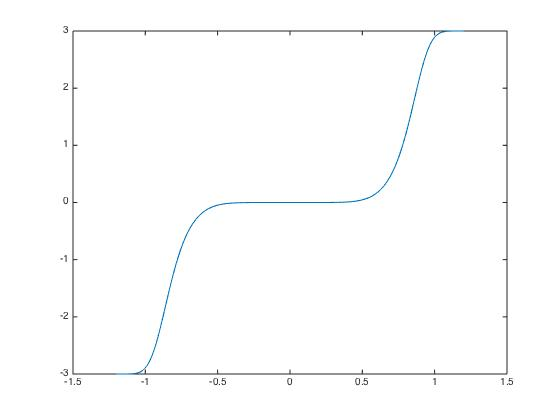
\includegraphics[height=5.7cm]{Acceleration.jpg}
\caption{Acceleration}
\end{figure}
\\
As for self-driving vehicles, since they can detect others' acceleration, if the acceleration of the vehicle ahead changes suddenly, self-driving cars will simultaneously change its acceleration so as to adapt.\\
%formula
\subsection{Merging and Divergence}
In reality, the number of lanes in a road is not constant,so sometimes vehicles need to merge into fewer lanes and sometimes diverge to more lanes. We assumed that
\subsection{Dedicating Lanes for Self-driving Vehicles}
The most significant difference between the self-driving vehicles and ordinary cars are reaction time and corporation between vehicles, which causes the self-driving cars running more smoothly. When the percentage of self-driving vehicles reaches some value, a special lane for self-driving vehicles could be dedicated in order to raise transportation efficient.

\section{Calculating and Simplifying the Model}
%theory of algorithm (figure)
A dynamic array is the foundation of the implementation, allowing multiple simulations on various percentage of  self-driving vehicles or various traffic volume. In order to simulate the structure of the model, firstly, a class $Car$ was  defined to store the information such as velocity, acceleration, serial Number etc. of a car, a dynamic array representing all positions cars may occupy was created, within which each
\begin{figure}[!htp]
\centering
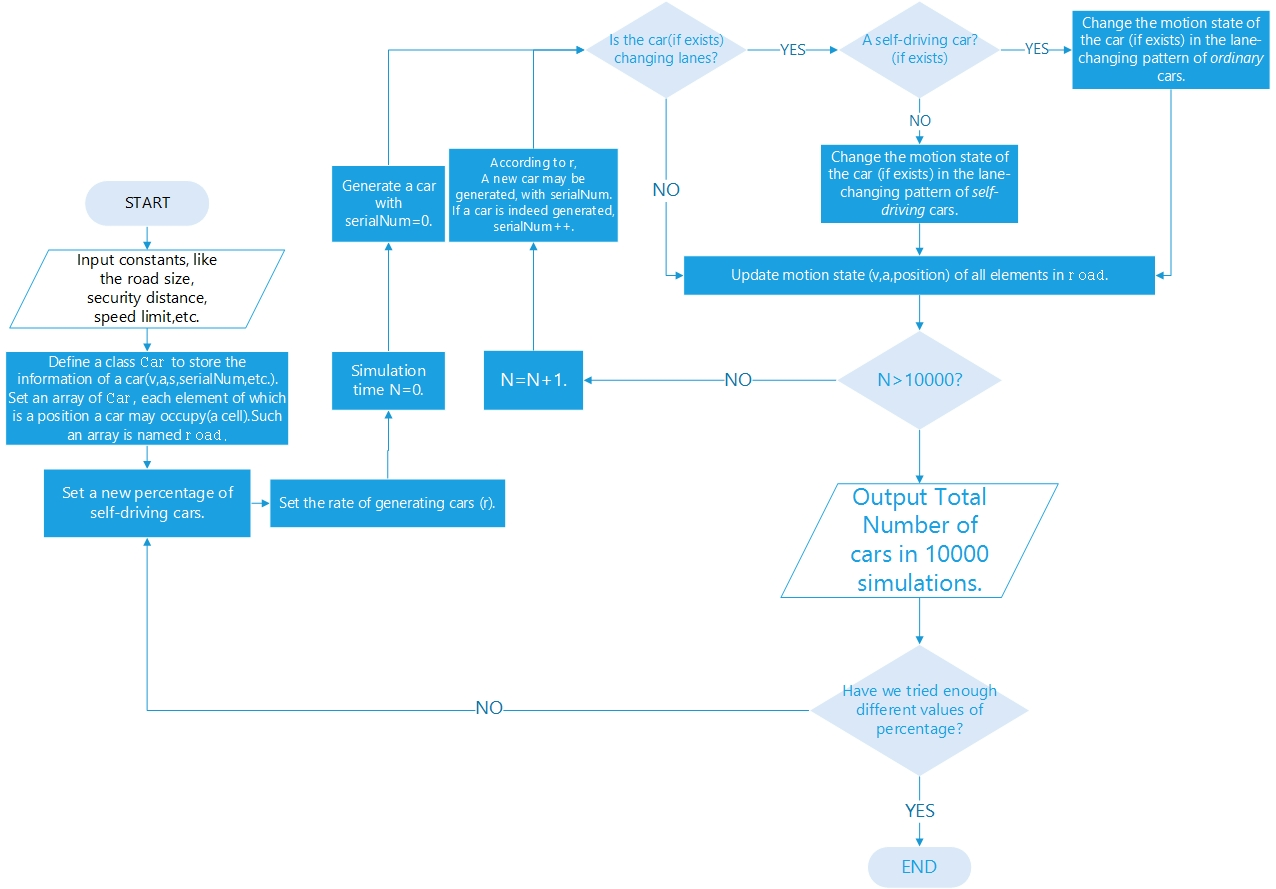
\includegraphics[height=11.1cm]{FlowChart1.jpg}
\caption{Flow Chart}
\end{figure}
\section{Revise and Improve the Model}
\subsection{Influence of merge and divergence}
There are more than one lanes on highway, and number of lanes changes at joints, so the vehicles must merge or diverge at these joints. This process will effect the velocity and acceleration of vehicles, thus causing a noticeable influence on traffic flow. In order to take this effect into account, we designed the following algorithm:\\
\subsection{Influence of cooperation between self-driving cars}
The cooperation system of self-driving cars makes the motion status transparent among self-driving vehicles, which may influence the strategy while merging/diverging. By qualitative analysis, a conclusion could be drawn that the self-driving vehicles tend to gather as a whole,
\section{Application of the Model}%apply to roads of interest
We input the data provided in the excel to our program, 
\section{The Model Results}
\subsection{Influence on Capacity of Percentage of self-driving vehicles}
To implement the traffic flow of a 1000-meter straight highway which has 5 lanes, we assume that 1 lane is set for self-driving cars. We make a policy that self-driving cars can run on any lane, but human-driving cars are not allowed to run on self-driving lane. We assume that a car will be generated at origin every 2.5 seconds, firstly we set the percentage of self-driving car to be 20$\%$, we use $\Delta N$ = $N_{1}$ - $N_{2}$ to measure the capacity of our model in 1000 seconds.%the statistics showed that the motion status of the whole  road will become steady after around 14 seconds, that is, after 14 seconds, for any certain point on the road, the velocities of vehicles when they pass through the point will be almost the same, this status is as shown in figure:\\
Then we adjust the percentage to 60$\%$, 90$\%$,the xxx are as shown:\\
\\
By statistics above, conclusion can be drawn that 
\subsection{Influence of cooperation between self-driving cars}
The self-driving cars own a cooperation system that can exchange information among each other, then we assume that .For %include figures:1.+Delta a, 2, no Delta a

\section{Conclusions}
\section{Evaluation of the Model}
\subsection{Strengths}
\begin{enumerate}
\item 
\end{enumerate} 
\subsection{Weakness}
\begin{enumerate}
\item We set the reaction time to be constant, but actually the reaction time of each driver at different time may vary, which may lead to error.
\item We used a formula to determine the accelerations of ordinary cars, but in reality, drivers cannot react so accurately, so an uncertain error may occur.
\item In our model, the accelerations of self-driving vehicles change instantaneously. This may harm smoothness of the system.
\item Overtaking is not considered in our model. If overtaking is allowed, the accelerations of vehicles will be influenced also by motion of vehicles in adjacent lanes.
\item In the formula of acceleration, we assumed that accelerations range from -3(m/$s^{2}$) to 3 (m/$s^{2}$), where sharp changes of acceleration are not considered, so this model can't be applied to extreme cases such as collision.
\end{enumerate}



%%% ---------------
%%% Bibliography

%\nocite{*}   %%% Include everything in the thesis.bib file.  Be
             %%% careful---some journals and fields expect you to only
             %%% include references for materials that you have
             %%% actually cited in your paper, others allow you to
             %%% include materials you used as ``background'' without
             %%% actually citing specific pages or passages.

%%% Feel free to choose any bibliography style you like.
\bibliographystyle{plainnat}
%%% The filename (without the bib extension) of your bibliography file.
\bibliography{icmmcm}

\end{document}




%%% Local Variables:
%%% mode: latex
%%% TeX-master: t
%%% End:
